\documentclass[12pt]{article}

%%%%%%%%%%%%%%%%%%%%%%%%%%%

\usepackage{graphicx} % Required for inserting images

%%%%%%%%%%%%%%%%%%%%%%%%%%
% Customize section heading to 14pt: do not modify
\usepackage{titlesec} % Used to set section heading font size
\titleformat{\section}
{\fontsize{14}{16}\selectfont\bfseries} % Format: size and style
{\thesection}     % Section number
{1em}             % Space between number and title
{}
% Load the setspace package
\usepackage{setspace}
% changes the text to double-line spacing - do not modify
\doublespacing
%load page sizing package
\usepackage[margin=2.54cm]{geometry} %Margin size - do not modify
% line spacing
\setstretch{1.45}  % do not modify
% Font choice - do not modify
\usepackage{mathptmx}
%%%%%%%%%%%%%%%%%%%%%%%%%%%%%%%%%%%%%%%%%%%%%%%%%%%%

%%%%%%%%%%%%%%%%%%%%%%%%%%%%%%%%%%%%%%%%%%%%%%%%%%%%
% Added packages. These do not alter the font, margins, spacing or heading
% sizes fixed above; they provide citations, tables, algorithms and code.
\usepackage{natbib}          % \citep and \citet, works with apalike
\usepackage{booktabs}        % rules for the result tables
\usepackage{algorithm}       % numbered algorithm floats
\usepackage{algpseudocode}   % pseudocode body
\usepackage{subcaption}      % multi-panel figures
\usepackage{url}             % apalike emits \url
\usepackage{tikz}            % Figures 2 and 3 are drawn, not imported
\usetikzlibrary{positioning, arrows.meta, fit, backgrounds}
\usepackage[T1]{fontenc}
%%%%%%%%%%%%%%%%%%%%%%%%%%%%%%%%%%%%%%%%%%%%%%%%%%%%

\begin{document}

%%%%%%%%%%%%%%%%%%%%%%%%%%%%%%%%%%%%%%%%%%%%%%%%%%%%%%%%%%%%%%%%%%%%%%%%%%%%%%%%%%%%%%%%%%%%%%%%%%%%%%%%%%%%%%%%%%
%%%%%%%%%%%%%%%%% Do not alter the latex commands in this title/abstract/acknowledgement generation %%%%%%%%%%%%%%
\begin{center}
\vspace*{4cm}
	{\Huge \bf{ Silent Failures in LLM-Generated CUDA Kernels } }\\
\vspace{2.5cm}
	{\LARGE \bf{ Ali Ansari } }\\
\vspace*{12cm}

Dissertation report submitted for the MSc Dissertation Module, \\
School of Computing Sciences, University of East Anglia, 2025/26
\end{center}

\newpage

\vspace{5cm}
\noindent {{\huge \bf Abstract}}\\
%%%%%%%%%%%%
% TODO: no more than 200 words. Draft in docs/writing-style.md.
Insert your abstract here. No more than 200 words.
%%%%%%%%%%%%%

\newpage
\vspace{5cm}

\noindent {{\huge \bf Acknowledgement }}\\
%%%%%%%%%%%%%%%%%%%%%
% TODO: no more than 200 words.
Insert your acknowledgement here. No more than 200 words.
%%%%%%%%%%%%%%%%%%%%%
%%%%%%%%%%%%%%%%%%%%%%%%%%%%%%%%%%%%%%%%%%%%%%%%%%%%%%%%%%%%%%%%%%%%%%%%%%%%%%%%%%%%%%%%%

%%%%%%%%%%%%%%%%%% insert a table of contents starting on a new page
\newpage

\tableofcontents

%%%%%%%%%%%%%%%%%% start a new page after your table of contents ends
\newpage

%%%%%%%%%%%%%%%%%%%%%%%%%%%%%%%%%%%%%%%%%%%%%%%%%%%%%%%%%%%%%%%%%%%%%%%%%%%%%%%%
% 1. INTRODUCTION -- 3 pages
%%%%%%%%%%%%%%%%%%%%%%%%%%%%%%%%%%%%%%%%%%%%%%%%%%%%%%%%%%%%%%%%%%%%%%%%%%%%%%%%
\section{Introduction}
% TODO 3 pages. Rubric: broad background; motivation and application;
% explicit statement of aim and objectives.
% Hook: AI systems now generate part of their own infrastructure.
% Reuse the phrase "correct, or merely harder to catch".

\subsection{Motivation}

Machine learning now depends on a small amount of code that almost nobody
writes. A GPU kernel is the layer where a mathematical operation becomes
instructions on hardware, and the performance of every model trained or served
today rests on a library of them. Writing one well takes expert knowledge of
memory hierarchies and thread scheduling, and the work is slow. FlashAttention,
one of the most consequential kernels of the last decade, arrived five years
after the architecture it accelerates \citep{dao2022flashattention,
ouyang2025kernelbench}.

This makes kernel generation an obvious target for language models, and the
field has moved quickly. Systems now translate PyTorch modules into CUDA,
search for faster variants, and train against measured speedup
\citep{li2026cudal1, dai2026cudaagent}. There is something recursive about the
result: models are beginning to write the infrastructure that runs models.

Every one of these systems shares a component and a blind spot. The component
is a repair loop. When a generated kernel fails, the error is returned to the
model and another attempt is requested, and this simple idea reliably raises
benchmark scores. The blind spot is what counts as failure. A kernel is judged
by comparing its output against a reference implementation on a few randomly
drawn inputs, and a kernel that is wrong in a way those inputs do not reach
will be recorded as correct.

Put those two facts together and an uncomfortable possibility appears. If a
model is repeatedly asked to fix the failures a test can see, it may learn to
produce kernels whose failures the test cannot see. The benchmark would report
progress either way.

This dissertation asks whether that happens. The question matters because a
kernel is a drop-in replacement for a component that already worked. A loud
failure costs an engineer an afternoon. A silent one returns plausible numbers
for as long as nobody checks.

\subsection{Aim and objectives}
\label{sec:aim}

The aim of this project is to determine whether iterative repair of
LLM-generated CUDA kernels improves their correctness, or merely conceals their
faults from the benchmark that scores them.

The objectives are:

\begin{enumerate}
\item Build a classifier that separates kernels which satisfy KernelBench's
correctness check from those which are correct under stronger testing, and
validate it against kernels of known category.
\item Design a stress battery of metamorphic probes that can be withheld from
the model, so that a repair loop cannot be optimised against it.
\item Measure the false-pass rate before and after repair, across several
models, both reasoning settings and two GPU architectures.
\item Determine whether repair changes how the benchmark ranks models.
\item Release the classified dataset and the analysis code so that every
reported number can be reproduced.
\end{enumerate}

This aim is narrower and sharper than the one in the original proposal, which
set out to build a general taxonomy of correctness failures. The taxonomy was
built, and it appears in Section~\ref{sec:taxonomy}, but it turned out to be a
means rather than an end: the interesting result was not the distribution of
failure types but the movement between them under repair. I have stated the aim
as the project actually developed.

\subsection{Terminology}
\label{sec:terminology}

Several terms in this report are either borrowed from software testing or
introduced here, and are used from Chapter~2 onwards. They are collected below
so that no definition arrives after its first use. The five failure categories
have their own table in Section~\ref{sec:taxonomy} and are not repeated here.

\begin{description}

\item[Reference module] The original PyTorch implementation that a generated
kernel is asked to replace. It defines what the kernel is supposed to compute,
because no other specification exists.

\item[Oracle] The procedure that decides whether a test has revealed a fault.
KernelBench's oracle compares the kernel's output against the reference module
on five random inputs. Every oracle is incomplete, in the sense that it can
only inspect the inputs it is given.

\item[Probe] One test in the stress battery. A probe transforms the input in a
specific way, runs both the reference module and the kernel on the transformed
input, and reports whether they still agree.

\item[Stress battery] The full set of probes, run only after a kernel has
already satisfied KernelBench's own check. The battery is the stronger oracle
this work adds.

\item[Metamorphic relation] A transformation of an input paired with the effect
it should have on the output. Every probe encodes one. Because a kernel must
behave like the module it replaces, the expected effect is always that the
output does not change.

\item[Arm] One of the two experimental conditions. The \emph{think} arm runs
the model with reasoning enabled; the \emph{direct} arm runs the same model,
with the same prompt, and reasoning disabled.

\item[Turn] A single request to the model. Turn~0 is the first attempt at a
problem, and turns 1 to 3 are repair attempts that follow a failure.

\item[Chain] The sequence of turns for one problem, in one arm, on one GPU. A
chain ends when the kernel passes, when it is judged silent, or after the
third repair turn.

\item[Visible failure] A kernel that fails in a way KernelBench can see:
\texttt{syntactic}, \texttt{runtime} or \texttt{functional}. These are the
failures reported back to the model during repair.

\item[Silent failure] A kernel that satisfies KernelBench's check and is
nonetheless wrong, because at least one probe in the battery disagrees with the
reference module. KernelBench scores such a kernel as a success.

\item[False-pass rate] Among the kernels KernelBench would report as correct,
the proportion that are in fact silent failures. Written as
$\mathit{silent} / (\mathit{silent} + \mathit{pass})$. This is the study's
central measurement.

\item[Relocation] The effect this dissertation reports: a repair turn converts
a visible failure into a silent one. The benchmark records the change as a
successful repair, because the failure it could see has gone.

\item[Strict and extended readings] Two ways of counting a silent failure. The
\emph{strict} reading condemns a kernel only when it violates KernelBench's own
stated contract. The \emph{extended} reading condemns any kernel that fails to
behave like the module it replaces. Results are reported under both, and
Section~\ref{sec:limitations} explains why.

\end{description}

\subsection{Contributions}

\textbf{1. A withheld stress battery for generated kernels.} I extend
KernelBench's correctness check with seven metamorphic probes over memory
layout, magnitude, dtype and repeated execution, and keep their results out of
the repair prompt so that the model cannot fit them.

\textbf{2. Evidence that repair relocates failures.} Across three models and
two GPU architectures, iterative repair raises the pass rate and the share of
passing kernels that are silently wrong at the same time. Of the 244 chains
that repair turns into an apparent success, 79, almost one in three, are silent
failures.

\textbf{3. Evidence that repair destroys the benchmark's discriminating power.}
Under KernelBench's own contract the three models converge after repair to
between 91.5\% and 93.5\%, a statistical tie in every pairwise test, while the
stress battery still separates them and reverses their order.

\textbf{4. A quantified account of where the effect comes from.} 85\% of silent
failures are caught by one relation, that a kernel must not change its answer
when the same values arrive through different strides, and I report every
headline number under both a strict and an extended reading of correctness.

\textbf{5. An open dataset and a reproducible pipeline.} 2{,}852 classified
kernel attempts, 1{,}196 repair chains and the generated sources, from which
every figure and table in this report regenerates by running one script.

\subsection{Report structure}

Chapter~2 reviews how kernel generation is evaluated, why test suites define
correctness rather than measure it, and what is known about repair loops, and
ends with the gap this work fills. Chapter~3 sets out the experimental design,
the failure taxonomy, the stress battery and the repair loop. Chapter~4
describes the implementation and how it was validated. Chapter~5 reports the
results. Chapter~6 states the limitations, and Chapter~7 concludes.

%%%%%%%%%%%%%%%%%%%%%%%%%%%%%%%%%%%%%%%%%%%%%%%%%%%%%%%%%%%%%%%%%%%%%%%%%%%%%%%%
% 2. LITERATURE REVIEW -- 5 pages
%%%%%%%%%%%%%%%%%%%%%%%%%%%%%%%%%%%%%%%%%%%%%%%%%%%%%%%%%%%%%%%%%%%%%%%%%%%%%%%%
\section{Literature Review}

\subsection{Writing code and checking it}

Large language models write useful code. Codex demonstrated this first, and it
also fixed how the field measures success: generate a program from a
description, run the tests that come with the task, and report the fraction
that pass \citep{chen2021codex}. That method works because the task carries its
own definition of correctness. The docstring states what the function should
do, and the tests check whether it does it.

CUDA kernels break this arrangement in two ways.

The first is widely recognised. A kernel is written against a particular memory
hierarchy and thread model, so good performance depends on hardware knowledge
that the source code never states \citep{kirk2012programming}. FlashAttention
illustrates the cost. It is an attention kernel that reduces traffic between
levels of GPU memory, and it required years of expert effort
\citep{dao2022flashattention}. \citet{ouyang2025kernelbench} observe that it
appeared five years after the Transformer was proposed, and needed two further
years to reach a new generation of GPUs.

The second difficulty attracts less attention, and it is the subject of this
dissertation. A kernel has no docstring. It is not written against a
specification that a test can consult. It is written to replace an existing
PyTorch module, so the only available definition of correct is ``behaves like
that module''. Comparing two implementations on every possible input is
impossible. In practice somebody selects a small number of inputs and compares
the outputs on those.

The choice of inputs therefore decides what correctness means.

\subsection{How KernelBench decides that a kernel is correct}
\label{sec:evaluated}

KernelBench is the standard benchmark for this task
\citep{ouyang2025kernelbench}. It supplies 250 PyTorch modules across three
difficulty levels and asks the model to return an equivalent module built
around a custom CUDA kernel. It then reports $\mathrm{fast}_p$: the share of
generated kernels that are correct and at least $p$ times faster than PyTorch.
Frontier reasoning models beat the PyTorch baseline in fewer than 20\% of
cases, so the benchmark is far from solved.

The correctness half of that score rests on a single procedure. The authors
``evaluate on 5 random inputs per problem'', checking ``equivalence of output
between reference architecture \texttt{Model} and generated architecture with
custom kernel \texttt{ModelNew}''.

They explain the choice openly. Proving two programs equivalent is undecidable,
so they adopt random testing, which they describe as ``the most common
practical approach''. They argue that it suits this domain, because AI kernels
have simple control flow and ``the focus is primarily on numerical
correctness''. Five inputs are presented as ``a good tradeoff between the
ability to catch errors and efficiency''. To justify that number they ran an
experiment on 100 generated kernels, and found that kernels either passed
everything or failed everything: ``the 0/5 and 0/100 failures indicate that no
partial correctness was observed''.

That experiment is where the argument weakens. Every input in it shares one
shape and one memory layout, and only the values inside the tensors change. A
kernel whose fault depends on layout rather than on values will therefore pass
all five draws, and all one hundred. The absence of partial correctness follows
from the way the inputs were sampled. It is not evidence that five inputs are
sufficient.

Two recent papers approach this point without reaching it.
\citet{lange2025robustkbench} report that existing kernel benchmarks ``suffer
from exploitable loopholes and insufficient diversity in testing conditions'',
and respond with a stricter benchmark of their own. \citet{li2026cudabeaver}
show that a model can satisfy the tests ``with repair by degeneration,
simplifying the CUDA code into a safer but slower program''. Both establish
that the score can be gamed. Neither asks the simpler question: how often is
the score merely wrong?

\subsection{Tests do not measure correctness, they define it}
\label{sec:oracle}

Software engineering has a name for the difficulty reached at the end of the
last section. A test oracle ``determines whether a test execution reveals a
fault, often by comparing the observed program output to the expected
output'', and building a complete one is ``recognised as one of the fundamental
challenges of software testing'' \citep{segura2016metamorphic}. KernelBench's
five inputs are an oracle in exactly this sense. The useful question is not
whether the oracle is imperfect, since its authors say as much, but how much it
misses.

\citet{liu2023evalplus} measured that for Python. They took HumanEval and
increased its test cases by a factor of eighty, then re-evaluated 26 models on
the extended version. The additional tests caught ``significant amounts of
previously undetected wrong code'' and reduced pass@k by up to 19.3--28.9\%.

The more troubling result concerns the ranking. Two models that lost to ChatGPT
on the original benchmark defeated it on the extended one. A weak oracle does
not flatter every model by the same amount. It reorders them.

Metamorphic testing offers a disciplined way to add tests when the correct
answer is not known in advance. Instead of checking a single output, it
transforms the input and observes how the output ``morphs'' in response
\citep{segura2016metamorphic}. For a kernel offered as a drop-in replacement,
one such relation is almost too obvious to state: the same values, presented
through a different memory layout, must produce the same result. No kernel
benchmark applies it.

\citet{ludwig2026kaizen} show what happens when somebody applies it in a
neighbouring setting. Testing LLM-translated CUDA-to-OpenMP code, they found
faults in programs ``that compile and pass developer-written tests yet produce
incorrect scientific results'', and report that these faults ``are often
input-dependent''. Their subject is translation rather than generation, and
they use no repair loop, but the failure mode is the one measured here.

That failure mode already has a name outside software testing. Studies of large
server fleets describe corruptions in which ``the only symptom is an erroneous
computation'' \citep{hochschild2021cores}. I adopt the same word, silent, for a
kernel that passes the benchmark and returns the wrong answer.

\subsection{Repair loops and the signal they learn from}
\label{sec:repair}

If a program fails, show the model the error and ask again.
\citet{chen2024selfdebug} formalised this idea, teaching a model to inspect
execution results and explain its own code, and reported improvements of up to
12\% on benchmarks that provide unit tests. \citet{madaan2023selfrefine}
generalised it to any task, using a single model as generator, critic and
reviser, and reported roughly 20\% absolute improvement across seven tasks.
Results of this kind are why repair is now a standard component rather than an
experiment.

Three later studies complicate the picture.

\citet{olausson2024selfrepair} charged repair its real cost. Each turn is
another model call, so the fair comparison is against simply drawing more
candidates. Judged that way, the gains are ``often modest, vary a lot between
subsets of the data, and are sometimes not present at all''. They locate the
reason in the feedback itself: repair is limited by ``the model's ability to
provide feedback on its own code'', and improves sharply when a stronger model
supplies that feedback.

\citet{huang2024cannot} go further. Without external feedback, models
``struggle to self-correct their responses'', and at times become worse. They
then explain where earlier positive results came from. Those experiments used
oracle labels to guide the correction, and ``the improvements vanish when
oracle labels are not available''.

\citet{brown2024monkeys} arrive at a compatible conclusion from a different
direction. Repeated sampling steadily raises the chance that some attempt is
correct, across four orders of magnitude. That coverage converts into real
performance only ``in domains like coding and formal proofs, where answers can
be automatically verified''.

Taken together, these three make one point. A repair loop can be no better than
the judge it answers to.

The kernel generation systems adopt repair without revisiting that judge.
CUDA-L1 rewards speedup through reinforcement learning, Astra runs several
agents through generation, testing and profiling, Kernel-Smith evolves a
population of candidates using ``structured execution feedback on compilation,
correctness, and speedup'', and CUDA Agent trains against ``automated
verification and profiling to provide reliable reward signals''
\citep{li2026cudal1, wei2025astra, cao2026ksearch, du2026kernelsmith,
dai2026cudaagent, chen2025cudallm}. Reasoning models, which work through
intermediate steps before answering \citep{wei2022cot}, perform best throughout.

What every one of these systems feeds back is the same short list: whether the
code compiled, whether it crashed, how fast it ran, and whether it matched the
reference on the standard inputs. None of them feeds back anything about memory
layout.

\subsection{The gap}

Two lines of work meet in this dissertation, and they have not met before.

Every recent CUDA kernel system repairs, returning compiler errors and failed
comparisons to the model and asking again. Software testing has argued for
decades that such comparisons are incomplete oracles, and that adding tests to
a benchmark exposes code that was wrong from the start.

\citet{lange2025robustkbench} showed that KernelBench's oracle can be
exploited. \citet{li2026cudabeaver} showed that a model can satisfy it by
making the kernel worse. Neither measured what repair does to correctness
across several turns.

So the question remains unasked. When a model repairs its own kernel, does the
kernel become correct, or only harder to catch? I measure that.

%%%%%%%%%%%%%%%%%%%%%%%%%%%%%%%%%%%%%%%%%%%%%%%%%%%%%%%%%%%%%%%%%%%%%%%%%%%%%%%%
% 3. DESIGN -- 8 pages
%%%%%%%%%%%%%%%%%%%%%%%%%%%%%%%%%%%%%%%%%%%%%%%%%%%%%%%%%%%%%%%%%%%%%%%%%%%%%%%%
\section{Design}

\subsection{Research design}

Section~\ref{sec:repair} ended with a prediction. A repair loop can be no
better than the judge it answers to, and every kernel system answers to a judge
that Section~\ref{sec:oracle} shows to be incomplete. This chapter describes an
experiment built to test that prediction.

The experiment needs three things, and no existing harness provides them
together.

First, it needs a correctness check stronger than the benchmark's. Without one,
a kernel that is wrong cannot be told apart from a kernel that is right.

Second, that stronger check must be hidden from the model. If the model can see
it, the model will repair against it, and the measurement collapses.

Third, the same kernel must be measured before and after repair. Only then can
a change be attributed to repair rather than to chance in a fresh sample.

The design below provides all three. KernelBench's own check is kept exactly as
it is, and treated as the benchmark's verdict. A battery of further checks is
added, and is never shown to the model. A repair loop then runs, driven only by
the benchmark's verdict, and every intermediate kernel is recorded.

One further control shapes the whole study. Comparing a reasoning model with a
non-reasoning model would confuse reasoning with everything else that differs
between two checkpoints: training data, size, tokeniser, alignment. I avoid
this by running two arms on the same model. Both arms use the same prompt and
the same temperature. The only difference is the \texttt{reasoning\_effort}
parameter, set to \texttt{high} in one arm and \texttt{none} in the other. Any
gap between the arms can therefore be attributed to reasoning alone.

This contrast is stronger than the paired-checkpoint comparison used in most
earlier work. It is possible only because current models expose reasoning as a
runtime switch over fixed weights \citep{qwen2025qwen3}.

\subsection{A taxonomy of kernel failures}
\label{sec:taxonomy}

KernelBench reports one bit: correct, or not. That bit hides distinctions which
matter for diagnosis. I therefore classify every generated kernel into one of
five categories, shown in Table~\ref{tab:taxonomy}.

\begin{table}[h]
\centering
\begin{tabular}{ll}
\toprule
category & meaning \\
\midrule
\texttt{syntactic}  & does not build \\
\texttt{runtime}    & crashes, trips the sanitizer, or is too slow to evaluate \\
\texttt{functional} & runs, wrong answer on the standard input \\
\texttt{silent}     & passes the standard check, wrong under the stress battery \\
\texttt{pass}       & correct on the standard input and survives the battery \\
\bottomrule
\end{tabular}
\caption{The five failure categories. The first matching stage wins, so every
kernel receives exactly one label.}
\label{tab:taxonomy}
\end{table}

The categories are ordered, and the first one that matches wins. This makes
each label deterministic, because a kernel that fails to build is never also
tested for numerical accuracy. The order runs from the cheapest and most
visible failure to the most expensive and least visible. It is also the order
in which a developer would meet them.

\texttt{silent} is the category this dissertation exists to measure. A silent
kernel compiles, runs, and agrees with the reference module on the inputs
KernelBench draws. Under KernelBench it is a success, and it counts towards
$\mathrm{fast}_p$. It is nonetheless wrong.

The other four categories exist mainly so that \texttt{silent} can be separated
cleanly from them. The rest of this chapter explains how each label is
assigned.

\begin{figure}[htbp]
\centering
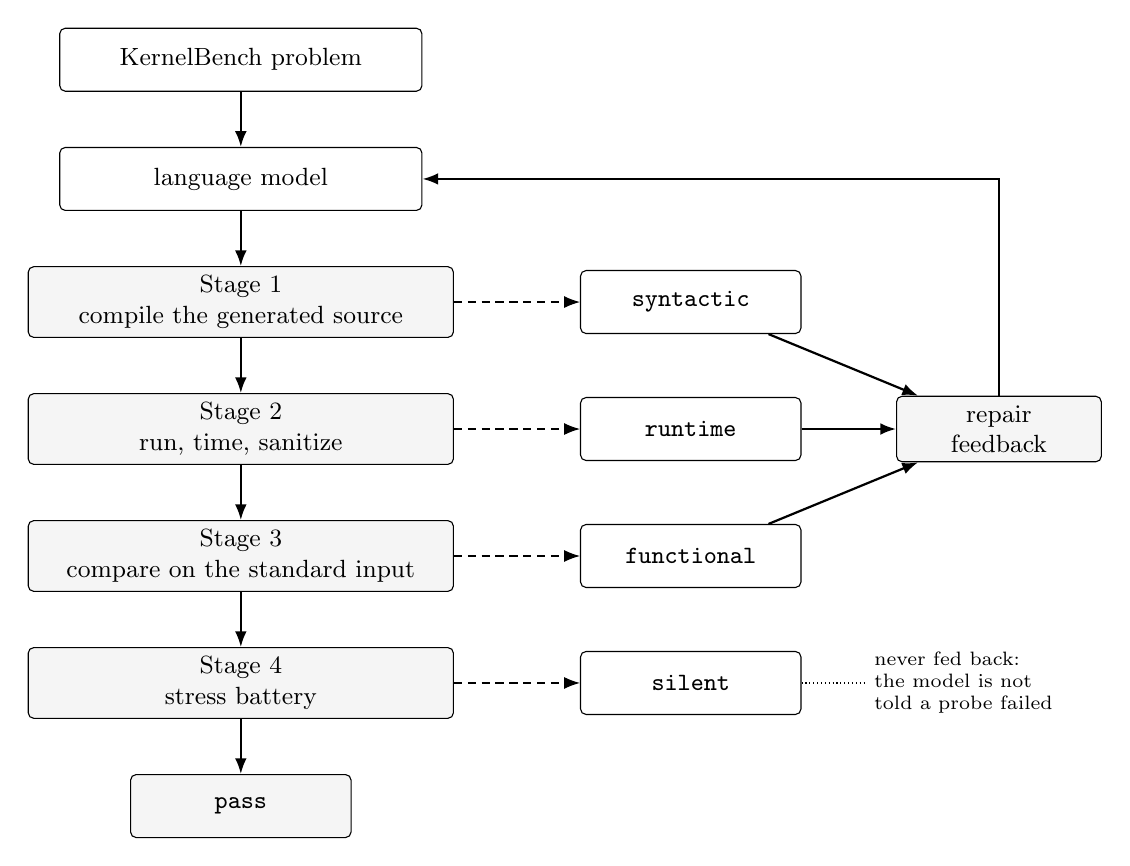
\begin{tikzpicture}[
  node distance=7mm and 16mm,
  every node/.style={font=\small},
  box/.style={draw, rounded corners=2pt, align=center,
              minimum height=8mm, inner xsep=3mm},
  stage/.style={box, fill=black!4, text width=48mm},
  cat/.style={box, text width=22mm, font=\small\ttfamily},
  good/.style={cat, fill=black!4},
  flow/.style={-{Latex[length=2mm]}, thick},
  fail/.style={-{Latex[length=2mm]}, densely dashed}
]

\node[box, text width=40mm] (prob) {KernelBench problem};
\node[box, below=of prob, text width=40mm] (llm) {language model};
\node[stage, below=of llm] (s1) {Stage 1\\compile the generated source};
\node[stage, below=of s1] (s2) {Stage 2\\run, time, sanitize};
\node[stage, below=of s2] (s3) {Stage 3\\compare on the standard input};
\node[stage, below=of s3] (s4) {Stage 4\\stress battery};
\node[good, below=of s4] (pass) {pass};

\node[cat, right=of s1] (syn) {syntactic};
\node[cat, right=of s2] (run) {runtime};
\node[cat, right=of s3] (fun) {functional};
\node[cat, right=of s4] (sil) {silent};

\draw[flow] (prob) -- (llm);
\draw[flow] (llm) -- (s1);
\draw[flow] (s1) -- (s2);
\draw[flow] (s2) -- (s3);
\draw[flow] (s3) -- (s4);
\draw[flow] (s4) -- (pass);

\draw[fail] (s1) -- (syn);
\draw[fail] (s2) -- (run);
\draw[fail] (s3) -- (fun);
\draw[fail] (s4) -- (sil);

\node[box, right=12mm of run, text width=20mm, fill=black!4] (rep)
  {repair\\feedback};
\draw[flow] (syn) -- (rep);
\draw[flow] (run) -- (rep);
\draw[flow] (fun) -- (rep);
\draw[flow] (rep.north) |- (llm.east);

\node[align=left, right=8mm of sil, text width=26mm, font=\scriptsize]
  (note) {never fed back:\\the model is not\\told a probe failed};
\draw[densely dotted] (sil.east) -- (note.west);

\end{tikzpicture}
\caption{The classification pipeline and the repair loop. A generated kernel
passes through four stages, and the first stage it fails determines its
category. Visible failures are returned to the model, which tries again for up
to three further turns. Stage 4 is deliberately excluded from that feedback, so
the model can never repair against the stress battery.}
\label{fig:pipeline}
\end{figure}

\subsection{The classifier}
\label{sec:classifier}

The classifier runs a fixed sequence of stages. Algorithm~\ref{alg:classify}
gives the sequence, and the rest of this section explains three decisions
inside it.

\begin{algorithm}[h]
\caption{Classifying one generated kernel}
\label{alg:classify}
\begin{algorithmic}[1]
\State seed the generator; build the reference model from the problem
\State \textbf{compile} the generated source \Comment{\texttt{load\_inline} builds here}
\If{compilation fails} \Return \texttt{syntactic} \EndIf
\State seed again; construct the candidate model with identical weights
\State run one forward pass on the standard input; \Call{synchronize}{}
\If{it raises} \Return \texttt{runtime} \EndIf
\State time one \emph{warm} forward call
\If{it exceeds the per-call budget} \Return \texttt{runtime} \EndIf
\State run \texttt{compute-sanitizer}
\If{a memory violation is reported} \Return \texttt{runtime} \EndIf
\State compare candidate and reference output on the standard input
\If{they disagree} \Return \texttt{functional} \EndIf
\State run the stress battery (Section~\ref{sec:battery})
\If{any probe disagrees} \Return \texttt{silent} \EndIf
\State \Return \texttt{pass}
\end{algorithmic}
\end{algorithm}

\textbf{Weight synchronisation.} Many Level 2 problems contain learnable
parameters. If the reference module and the candidate module are built from
different random draws, they hold different weights. Their outputs then differ
for reasons that have nothing to do with the kernel, and every kernel looks
wrong. Following KernelBench, I reseed the random generator three times: before
the initialisation inputs are produced, before each module is constructed, and
before every input draw. The two modules then hold identical weights and see
identical data. An early version of this work missed one of these reseeds, and
produced a false-pass rate that meant nothing.

\textbf{A budget per forward call.} One classification issues roughly ninety
forward calls, between the battery probes and the timing runs. A container time
limit is therefore really a budget per call. A kernel that needs tens of
seconds per call cannot finish inside the limit. Worse, it used to produce no
record at all, which quietly removed the slowest kernels from the dataset.
Stage 2a$'$ now times a single \emph{warm} call using CUDA events, and rejects
the kernel at once if it exceeds the budget. The call must be warm because the
first call also pays for lazy module loading and CUDA context setup, and is
not a fair sample.

The two limits are coupled. A T4 runs roughly 3.8 times slower than an L4, so a
budget that is correct on one device rejects kernels on the other for being
slow rather than for being wrong. The configuration refuses an inconsistent
pair rather than produce data that looks valid and is not.

\textbf{A comparison tolerance.} Outputs are compared with an absolute and
relative tolerance of $10^{-3}$, applied recursively through tuples, lists and
dictionaries so that structured returns are handled. The tolerance is a real
choice. Set it too tight, and ordinary floating-point reassociation is reported
as a fault. Set it too loose, and a genuinely wrong kernel passes.

\subsection{The stress battery}
\label{sec:battery}

The battery is the stronger oracle promised in the research design.

Each probe presents inputs that the standard check never uses. It then compares
the candidate against the reference on those same inputs. A probe can therefore
only fail when the two implementations disagree. This matters, because the
battery never holds its own idea of the right answer. It cannot punish a kernel
for anything except differing from the module it claims to replace.

Each probe encodes a metamorphic relation in the sense of
\citet{segura2016metamorphic}. Such a relation pairs a transformation of the
input with the expected effect on the output. Here the expected effect is
always the same: the output must not change. Table~\ref{tab:probes} lists the
probes.

\begin{table}[h]
\centering
\begin{tabular}{lll}
\toprule
probe & transformation & fault it exposes \\
\midrule
\texttt{fresh\_seed\_1..3}  & redraw the input values          & hardcoded or lucky outputs \\
\texttt{non\_contig}        & restride without changing values & assuming dense row-major layout \\
\texttt{nondeterministic}   & repeat the identical call        & races, reused internal buffers \\
\texttt{zeros}              & all-zero input                   & division by zero, uninitialised reads \\
\texttt{small\_magnitude}   & scale values down                & numerical instability \\
\texttt{extreme}            & scale values up                  & overflow, saturation \\
\texttt{fp16}               & halve the input precision        & dtype assumptions \\
\bottomrule
\end{tabular}
\caption{The stress battery. Every probe holds the reference implementation
fixed, and requires the candidate to agree with it on the transformed input.}
\label{tab:probes}
\end{table}

One probe deserves separate comment, because it dominates the results.
\texttt{non\_contig} builds a tensor holding exactly the same values as the
standard input, but presented through non-unit strides. It does this by
stacking the tensor with itself and taking one slice. A kernel that indexes raw
pointers, assuming a dense row-major layout, then reads the wrong elements and
returns a wrong answer. A kernel that calls \texttt{.contiguous()}, or respects
the strides it is given, returns the right one. KernelBench draws only
contiguous tensors, so this fault is invisible to it by construction.

Two rules keep the headline number honest. Both were added after early runs
produced figures that were wrong in the flattering direction.

The first rule is that a harness fault is never charged to the kernel. If a
probe raises because the machine ran out of memory, or because the harness
itself failed, the probe records \texttt{skipped} and the kernel is not
condemned. Before this rule, an out-of-memory error during the probes on a
16\,GB card turned working kernels into silent failures, and inflated the
study's headline metric.

The second rule is that refusing a dtype is not failing it. A kernel compiled
against \texttt{data\_ptr<float>()} cannot accept half-precision input, and
raises before a single thread runs. That is the kernel enforcing its declared
contract, not computing a wrong answer, so it is recorded as a robustness flag
rather than a silent failure. Before this rule every passing kernel carried an
\texttt{fp16} failure, and a probe that fires on all passing kernels measures
the harness rather than the kernel.

\subsection{The repair loop}

After a failure the model is shown its own source and the actual error, and
asked again. The loop runs for up to three further turns.

Only \texttt{syntactic}, \texttt{runtime}, \texttt{functional} and
\texttt{empty} are repairable, and \texttt{pass} and \texttt{silent} end the
chain. The feedback is deliberately plain: the compiler's own message, the
exception, or the reported numerical mismatch. Logs are truncated from the end,
because \texttt{nvcc} puts the decisive line last.

The most important decision in this design is what the loop is \emph{not}
told.

Stage 4 never appears in the feedback. A silent kernel ends its chain in
exactly the way a passing kernel does, and the model is never told that a
stress probe disagreed.

This is not a convenience. \citet{huang2024cannot} show that reported gains
from self-correction in earlier work came from oracle labels guiding the
process, and that those gains disappear once the labels are withdrawn. A stress
battery fed back into the prompt would be exactly such an oracle label. The
model would repair against it, the false-pass rate would fall, and that fall
would measure the model's skill at fitting a held-out test rather than any real
improvement in correctness. Withholding stage 4 keeps the battery an
independent instrument instead of part of the training signal, and it is what
makes the false-pass rate in Section~\ref{sec:relocation} meaningful.

The choice also matches deployment. A developer running a repair loop against
KernelBench sees compiler errors and failed comparisons. They do not see a
stress battery, because they do not have one.

\subsection{Experimental plan}

\textbf{Models.} Three models are evaluated: GLM-5, DeepSeek V3.2 and
Qwen3-235B-A22B, each served through Amazon Bedrock.

The selection criterion was not capability but controllability. The two-arm
design needs a model whose reasoning can genuinely be turned off. Several
otherwise suitable candidates reason regardless of the parameter, and those
were rejected: their \texttt{direct} arm would silently have been a second
\texttt{think} arm, and the central contrast would have been empty. This limits
generality, and I state it as a limit. The findings apply to models that expose
reasoning as a runtime switch.

\textbf{Tasks.} KernelBench Level 2, the fusion tier, in which several PyTorch
operators must be combined into one kernel. Level 1 is excluded because
single-operator problems are largely solved and produce too few failures to
analyse. Level 3 is excluded for time, and Section~\ref{sec:limitations}
returns to that exclusion. All 100 Level 2 problems are used, in ten stratified
batches of ten, so that a partial run still covers the full difficulty range.

\textbf{Hardware.} Every problem runs on two GPUs: an Ada-generation L4 and a
Turing-generation T4. Both use one pinned CUDA image and one pinned set of
Python packages. Running both makes it possible to detect a kernel that passes
on one architecture and fails on another, and guards against a result that is
an artefact of a single device.

\textbf{Determinism.} Temperature is zero, and one sample is drawn per problem,
per arm, per turn. Each cell of the design is therefore a single greedy
generation. This makes the experiment cheap and exactly reproducible, at the
cost of confidence intervals, and Section~\ref{sec:limitations} examines that
cost. The benchmark dataset is pinned to one revision, so later upstream edits
cannot change what was run.

The full design is 3 models $\times$ 2 arms $\times$ 2 GPUs $\times$ 100
problems $\times$ 4 turns. It is evaluated lazily: a chain stops as soon as it
reaches \texttt{pass} or \texttt{silent}.

%%%%%%%%%%%%%%%%%%%%%%%%%%%%%%%%%%%%%%%%%%%%%%%%%%%%%%%%%%%%%%%%%%%%%%%%%%%%%%%%
% 4. IMPLEMENTATION -- 5 pages
%%%%%%%%%%%%%%%%%%%%%%%%%%%%%%%%%%%%%%%%%%%%%%%%%%%%%%%%%%%%%%%%%%%%%%%%%%%%%%%%
\section{Implementation}

\subsection{System architecture}
\label{sec:architecture}

The system is organised around one rule: code that decides an outcome must be
testable without a GPU.

Everything in the \texttt{kfault} package is therefore pure Python. It makes no
API calls, touches no GPU, and opens no network connection. The classifier, the
stress battery, the output comparison, the repair feedback and the analysis all
live there. Only the scripts at the top level talk to Modal or to the model
provider. Table~\ref{tab:modules} lists the parts.

\begin{table}[h]
\centering
\begin{tabular}{ll}
\toprule
module & responsibility \\
\midrule
\multicolumn{2}{l}{\emph{\texttt{kfault/}: pure logic, no GPU or network}} \\
\texttt{classifier.py} & the four stages of Algorithm~\ref{alg:classify} \\
\texttt{battery.py}    & the stress probes \\
\texttt{comparison.py} & output comparison, tree mapping, cloning \\
\texttt{analysis.py}   & chains, distributions, false-pass rates \\
\texttt{benchmark.py}  & interleaved CUDA-event timing \\
\texttt{repair.py}     & repair feedback and repairable categories \\
\texttt{prompts.py}    & prompt construction and response parsing \\
\texttt{generation.py} & model calls and the generation cache key \\
\texttt{sanitizer.py}  & \texttt{compute-sanitizer} driver and output parsing \\
\texttt{cache.py}      & stable keys and atomic writes \\
\texttt{config.py}     & every tunable, and the guards between them \\
\texttt{report.py}     & formatting for the console summaries \\
\midrule
\multicolumn{2}{l}{\emph{top level: infrastructure}} \\
\texttt{pipeline.py}   & Modal app: generate, classify, repair \\
\texttt{validate.py}   & known-answer validation of the classifier \\
\texttt{export.py}     & cache to CSV and kernel sources \\
\texttt{figures.py}    & CSV to figures \\
\bottomrule
\end{tabular}
\caption{Module responsibilities. The horizontal rule marks the boundary
between logic that runs anywhere and code that needs Modal.}
\label{tab:modules}
\end{table}

The split exists for one practical reason. Because the classifier and the
battery carry no infrastructure, their behaviour can be checked on an ordinary
laptop. The 86 unit tests described in Section~\ref{sec:validation} run in four
milliseconds, with no GPU, no container and no cost. A design that mixed the
two would have made every logic change an experiment.

\begin{figure}[htbp]
\centering
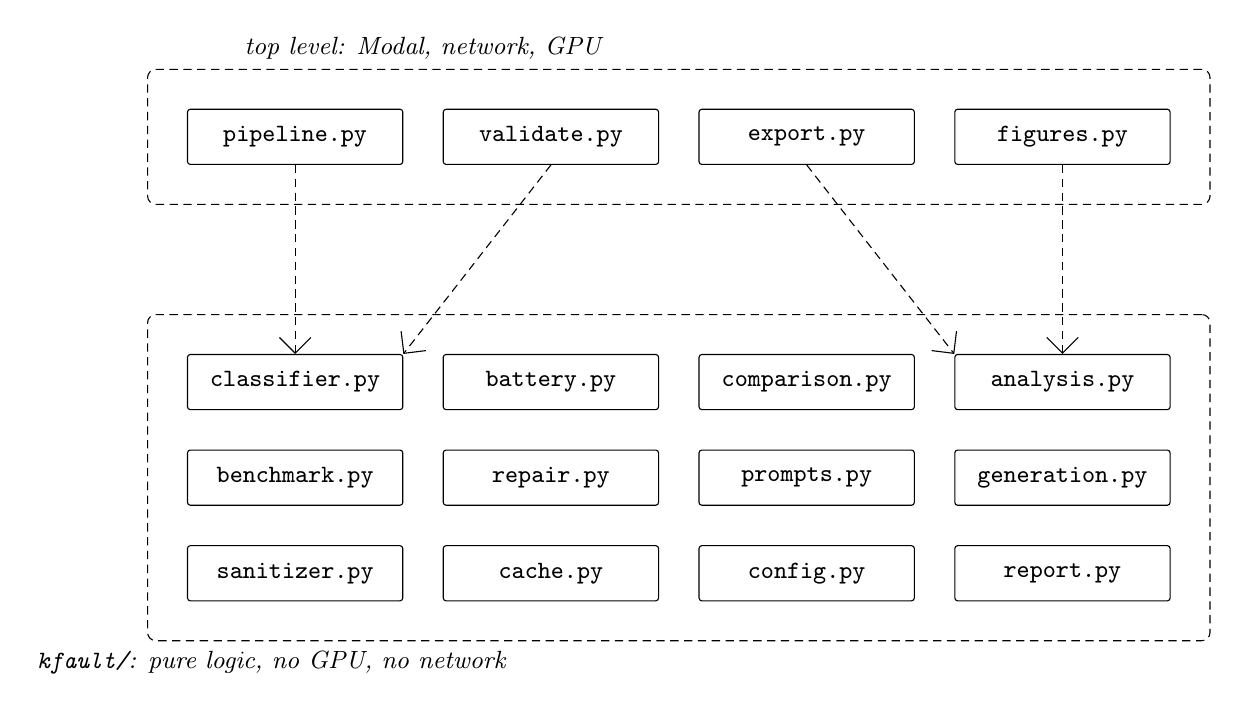
\begin{tikzpicture}[
  every node/.style={font=\small},
  comp/.style={draw, rounded corners=1pt, minimum height=7mm,
               text width=25mm, align=center, font=\small\ttfamily,
               fill=white},
  pkg/.style={draw, densely dashed, rounded corners=3pt, inner sep=5mm},
  dep/.style={-{Straight Barb[length=2mm]}, densely dashed}
]

% top-level scripts
\node[comp] (pipeline) {pipeline.py};
\node[comp, right=5mm of pipeline] (validate) {validate.py};
\node[comp, right=5mm of validate] (export) {export.py};
\node[comp, right=5mm of export] (figures) {figures.py};

% pure package: three rows, dependency targets on the first row
\node[comp, below=24mm of pipeline] (classifier) {classifier.py};
\node[comp, right=5mm of classifier] (battery) {battery.py};
\node[comp, right=5mm of battery] (comparison) {comparison.py};
\node[comp, right=5mm of comparison] (analysis) {analysis.py};

\node[comp, below=5mm of classifier] (benchmark) {benchmark.py};
\node[comp, right=5mm of benchmark] (repair) {repair.py};
\node[comp, right=5mm of repair] (prompts) {prompts.py};
\node[comp, right=5mm of prompts] (generation) {generation.py};

\node[comp, below=5mm of benchmark] (sanitizer) {sanitizer.py};
\node[comp, right=5mm of sanitizer] (cache) {cache.py};
\node[comp, right=5mm of cache] (config) {config.py};
\node[comp, right=5mm of config] (report) {report.py};

\begin{scope}[on background layer]
  \node[pkg, fit=(pipeline)(figures),
        label={[font=\small\itshape]above left:
        top level: Modal, network, GPU}] (top) {};
  \node[pkg, fit=(classifier)(analysis)(sanitizer)(report),
        label={[font=\small\itshape]below left:
        \texttt{kfault/}: pure logic, no GPU, no network}] (pure) {};
\end{scope}

\draw[dep] (pipeline.south)  -- (classifier.north);
\draw[dep] (validate.south)  -- (classifier.north east);
\draw[dep] (export.south)    -- (analysis.north west);
\draw[dep] (figures.south)   -- (analysis.north);

\end{tikzpicture}
\caption{Component structure, with dashed arrows showing UML dependencies.
They run in one direction only: the top-level scripts import the pure package,
and nothing in \texttt{kfault/} imports Modal, the model client or CUDA. Only
the principal dependency of each script is drawn; \texttt{pipeline.py} also
uses \texttt{cache}, \texttt{config}, \texttt{prompts} and \texttt{repair}.
This structure is what allows the classifier, the battery and the analysis to
be tested without a GPU.}
\label{fig:components}
\end{figure}

One module does not respect the rule. \texttt{pipeline.py} defines the
container image, looks up the cache, orchestrates the repair chain and provides
the command line, all in one file. It is the least cohesive part of the system.
Splitting the image definition from the orchestration would be the first change
I would make if the work continued.

\subsection{Execution environment}

Generated code is untrusted. A model asked for a CUDA kernel can return
anything, and that code is compiled and executed. Each classification therefore
runs in a single-use container with the network blocked and access to other
Modal resources withdrawn. The container is destroyed afterwards, so no
generated kernel can affect the next one.

Reproducibility requires the environment to be fixed rather than merely
described. The CUDA image is pinned by its SHA-256 digest rather than by tag,
because a tag can be repointed to a new build. The Python packages are pinned
to exact versions: \texttt{torch==2.6.0}, \texttt{ninja==1.11.1.1},
\texttt{openai==2.41.1}, \texttt{datasets==5.0.0} and \texttt{modal==1.5.0}.
The KernelBench dataset is pinned to one revision, so a later upstream edit
cannot silently change the problems.

Two settings deserve mention because they affect the numbers directly.

TF32 arithmetic is disabled for both matrix multiplication and cuDNN. Left on,
TF32 reduces precision in a way that differs between GPU generations, which
would have confounded the comparison between the L4 and the T4 in
Section~\ref{sec:crossgpu}. Disabling it makes a numerical disagreement
attributable to the kernel rather than to the hardware.

Every \texttt{KFAULT\_*} setting is baked into the image. Modal does not
forward local environment variables into containers, and the configuration is
read container-side, so a value set only in the local shell is ignored without
warning. Section~\ref{sec:validation} describes what that cost before it was
found.

\subsection{Caching and provenance}

Generation is expensive and classification is not. The two are therefore cached
under independent keys, which is what makes re-labelling affordable.

The \textbf{generation key} covers the model, the reasoning effort, the
problem, the sample index, the temperature, a hash of the prompt, and the
client library version. It deliberately excludes the GPU. The same kernel can
then be classified on both devices without being paid for twice, which is what
makes the cross-GPU comparison cheap enough to run at all.

The \textbf{classification key} covers the generation artefact, the seed, the
sanitizer flag, the GPU, the CUDA image, the pinned packages, the schema
version, and the per-call time budget when it differs from the default.

Behind both keys sits one principle: \emph{a field that decides an outcome must
be part of the key}. The per-call budget is the clearest case. It determines
whether a slow kernel is labelled \texttt{runtime} or goes on to a full battery
run, so two budgets must never share a cache entry. It is omitted from the key
when it holds its default value, which keeps entries written before the budget
existed valid.

The separation gives two distinct operations. \texttt{-{}-force} re-classifies
a kernel while reusing the stored model output, so a change to the battery
costs GPU time but no model calls. \texttt{-{}-regen} requests genuinely new
generations. Every result in this dissertation was produced with the schema
version recorded alongside it, so a record classified under an older battery
can be identified and re-run.

\subsection{Validation}
\label{sec:validation}

A classifier that assigns the wrong label produces confident and worthless
results. Validation therefore runs at two levels.

The first is 86 unit tests over the pure modules, covering the analysis
functions, the battery bookkeeping, the repair feedback, the prompt handling
and the cache keys. They need no GPU and complete in four milliseconds.

The second is known-answer validation. Eleven hand-written kernels of known
category are run through the real classifier on real hardware: correct kernels
with weights, with mutating inputs, with structured returns and with nested
inputs, plus one kernel each for \texttt{syntactic}, \texttt{runtime},
\texttt{functional} and \texttt{silent}, and one that is correct but too slow.
The silent case is a kernel that is right on contiguous input and wrong on
strided input, so it exercises the probe the results depend on most.

The check asserts the category and, where it matters, the failing stage.
\texttt{runtime} is reachable several ways, so a slow kernel could otherwise be
recorded as correct for the wrong reason.

This layer earned its cost. Three defects were found that would each have
corrupted the headline number, and all three passed the unit tests.

The first was silent in the strict sense. The routine that copies tensors
preserved their values but not their strides, so the \texttt{non\_contig} probe
was handing the kernel a contiguous tensor and testing nothing. Every
false-pass rate measured before the fix was measured with the study's main
probe disabled.

The second was the opposite failure. The \texttt{fp16} probe reported a crash
on every passing kernel, because a kernel compiled against
\texttt{data\_ptr<float>()} cannot accept half input at all. A probe that fires
on 100\% of cases carries no information; it measures the harness.

The third was environmental. Because \texttt{KFAULT\_GPU} was not forwarded
into the image, 70 records were labelled with the wrong device. The fix was to
read the device name on the GPU itself and treat that as ground truth, rather
than trusting a value the container may never have received.

\subsection{Reproducibility}

No figure or table in this report contains a hand-copied number. The cache is
exported to \texttt{attempts.csv} and \texttt{chains.csv}, together with 2{,}829
kernel source files; every figure is then generated from those files by one
script. Re-running that script reproduces the figures exactly, and the exported
dataset allows the analysis to be repeated without access to a GPU.

%%%%%%%%%%%%%%%%%%%%%%%%%%%%%%%%%%%%%%%%%%%%%%%%%%%%%%%%%%%%%%%%%%%%%%%%%%%%%%%%
% 5. EVALUATION -- 10 pages
%%%%%%%%%%%%%%%%%%%%%%%%%%%%%%%%%%%%%%%%%%%%%%%%%%%%%%%%%%%%%%%%%%%%%%%%%%%%%%%%
\section{Evaluation}

\subsection{Dataset and scale}

The experiment produced \textbf{2{,}852 classified kernel attempts} arranged
into \textbf{1{,}196 repair chains}, with no missing cells: every model was run
on every Level 2 problem, in both arms, on both GPUs. Table~\ref{tab:dataset}
gives the distribution of labels over all attempts.

\begin{table}[h]
\centering
\begin{tabular}{lrr}
\toprule
category & attempts & share \\
\midrule
\texttt{functional} & 1{,}114 & 39.1\% \\
\texttt{syntactic}  &   611 & 21.4\% \\
\texttt{pass}       &   582 & 20.4\% \\
\texttt{runtime}    &   341 & 12.0\% \\
\texttt{silent}     &   172 &  6.0\% \\
\texttt{empty}      &    23 &  0.8\% \\
\texttt{error}      &     9 &  0.3\% \\
\midrule
total               & 2{,}852 & \\
\bottomrule
\end{tabular}
\caption{Label distribution over all attempts, including intermediate repair
turns. \texttt{error} marks a harness fault rather than a property of the
kernel.}
\label{tab:dataset}
\end{table}

Two observations before the analysis. First, wrong answers outnumber build
failures: \texttt{functional} is the largest category. Writing CUDA that
compiles is easier than writing CUDA that computes. Second, 172 attempts are
silent, which is 6\% of all attempts but a much larger share of the attempts
that KernelBench would call correct. That share is the subject of
Section~\ref{sec:relocation}.

\subsection{Reasoning and the failure distribution}

Table~\ref{tab:passrates} reports the pass rate for each model and arm, before
and after repair.

\begin{table}[h]
\centering
\begin{tabular}{llrr}
\toprule
model & arm & one-shot & after repair \\
\midrule
GLM-5         & think  & 58.5\% & 74.5\% \\
GLM-5         & direct & 38.5\% & 47.5\% \\
DeepSeek V3.2 & think  & 41.2\% & 74.4\% \\
DeepSeek V3.2 & direct &  2.0\% &  5.6\% \\
Qwen3-235B    & think  & 66.5\% & 82.5\% \\
Qwen3-235B    & direct &  2.0\% &  7.0\% \\
\bottomrule
\end{tabular}
\caption{Pass rate per model and arm, out of 200 chains each (100 problems on
two GPUs). The arms differ only in whether reasoning is enabled.}
\label{tab:passrates}
\end{table}

Reasoning matters enormously. Two of the three models are close to unusable
without it: DeepSeek V3.2 and Qwen3-235B each solve 2\% of Level 2 problems on
the first attempt with reasoning disabled, against 41\% and 67\% with it
enabled. GLM-5 degrades more gracefully, but still loses twenty points.

This confirms what the benchmarks already report \citep{ouyang2025kernelbench,
zhu2026cudabench} and I claim no novelty for it. It matters here for one
reason only. The direct arm produces so few passing kernels that any rate
computed over them rests on a handful of cases, and I treat direct-arm
percentages with caution throughout. The reasoning arm carries the argument.

Figure~\ref{fig:taxonomy} shows how the whole distribution moves under repair
rather than the pass rate alone.

\begin{figure}[htbp]
\centering
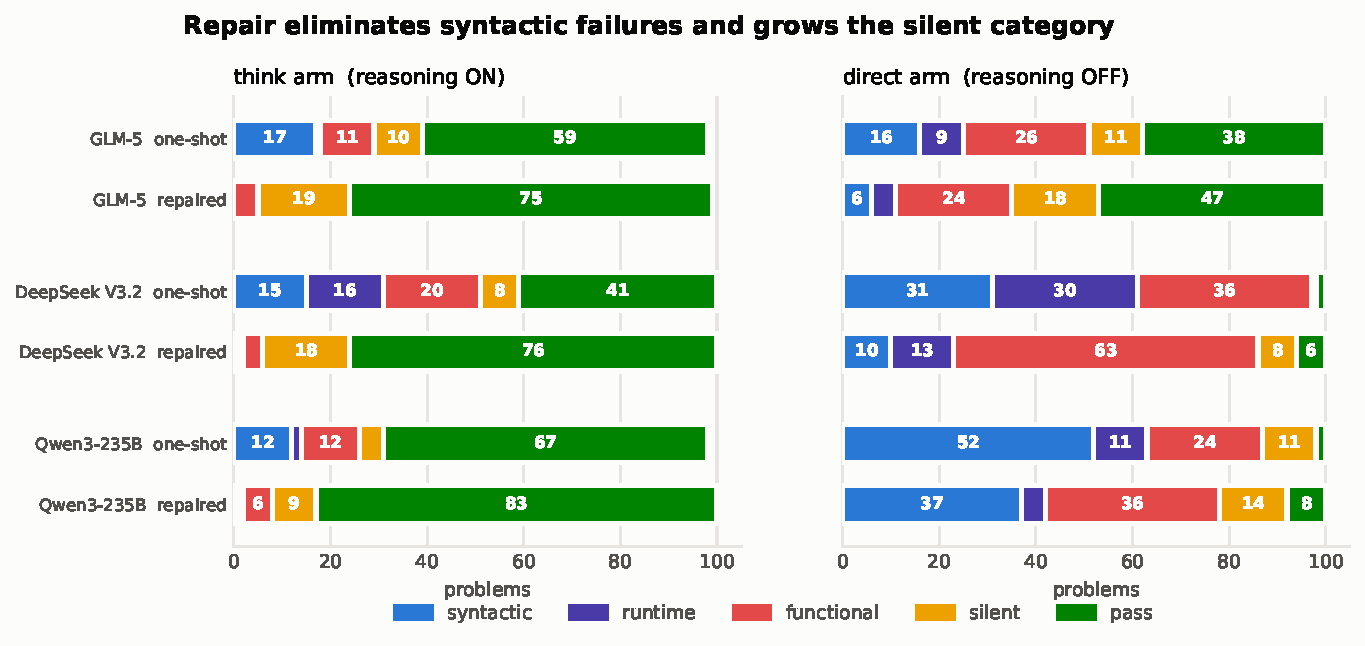
\includegraphics[width=0.92\linewidth]{figures/fig3_taxonomy.pdf}
\caption{Failure distribution before and after repair, for every model and arm.
Repair removes build failures very effectively. The \texttt{silent} band does
not shrink with them.}
\label{fig:taxonomy}
\end{figure}

\subsection{Repair relocates failures}
\label{sec:relocation}

Repair works, by the benchmark's own measure. It raises the pass rate in every
model and every arm, by as much as 33 points for DeepSeek V3.2 in the reasoning
arm. On that evidence a practitioner would adopt it without hesitation.

The false-pass rate tells a different story. Table~\ref{tab:falsepass} reports,
among the kernels KernelBench would accept, the share that fail the stress
battery.

\begin{table}[h]
\centering
\begin{tabular}{llrr}
\toprule
model & arm & one-shot & after repair \\
\midrule
GLM-5         & think  & 14.6\% (20/137) & \textbf{20.3\%} (38/187) \\
DeepSeek V3.2 & think  & 17.2\% (17/99)  & \textbf{19.6\%} (36/184) \\
Qwen3-235B    & think  &  7.0\% (10/143) & \textbf{9.8\%}  (18/183) \\
\midrule
GLM-5         & direct & 21.4\% (21/98)  & 26.4\% (34/129) \\
DeepSeek V3.2 & direct & 33.3\% (2/6)    & 59.3\% (16/27) \\
Qwen3-235B    & direct & 85.2\% (23/27)  & 67.4\% (29/43) \\
\bottomrule
\end{tabular}
\caption{False-pass rate, with counts, as silent over silent plus pass. In the
reasoning arm the rate rises for every model. Direct-arm denominators are small
and those rows should not be read as rates.}
\label{tab:falsepass}
\end{table}

In the reasoning arm the false-pass rate rises for all three models, by between
2.8 and 5.7 points. Figure~\ref{fig:relocation} shows the movement directly.

\begin{figure}[htbp]
\centering
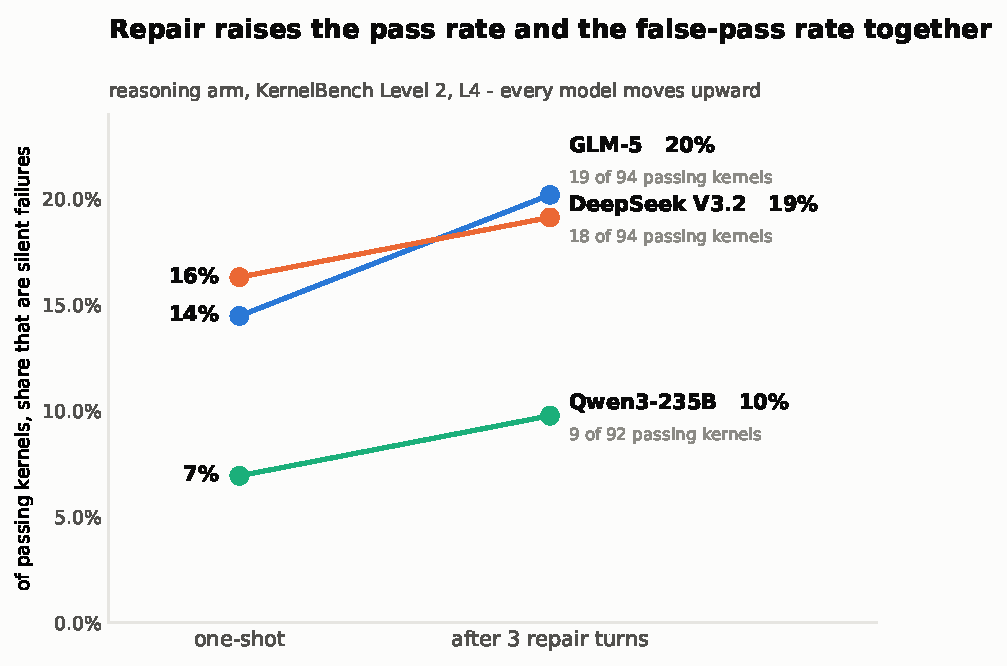
\includegraphics[width=0.9\linewidth]{figures/fig1_relocation.pdf}
\caption{Repair raises the pass rate and the false-pass rate together. Every
model moves upward, so a harness that reports only the pass rate records this
as unambiguous improvement.}
\label{fig:relocation}
\end{figure}

The direct arm is less clean and I do not lean on it. GLM-5 and DeepSeek V3.2
rise as expected, but Qwen3-235B falls, from 85.2\% to 67.4\%. With 27 passing
kernels at the start, a change of that size reflects a handful of individual
problems rather than a trend.

The mechanism is visible in the chains themselves. Counting outcomes across all
1{,}196 chains, repair rescued 165 chains to a genuine pass and converted
\textbf{79 chains from a visible failure into a silent one}. Those 79 are the
relocations. Combining the two gives the number a benchmark would report:

\begin{quote}
Repair produced 244 chains that KernelBench scores as a success. 79 of them,
\textbf{almost one in three}, are silent failures.
\end{quote}

The effect is not confined to one model. It appears in GLM-5 (32 chains),
DeepSeek V3.2 (33) and Qwen3-235B (14), and splits evenly across the two GPUs.
Figure~\ref{fig:outcomes} breaks the chains down by outcome.

\begin{figure}[htbp]
\centering
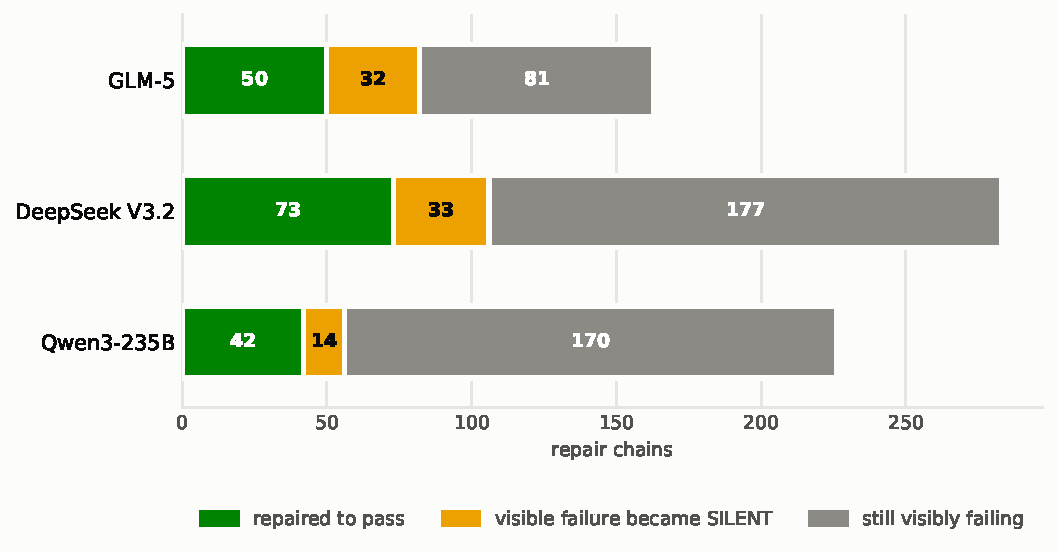
\includegraphics[width=0.92\linewidth]{figures/fig2_repair_outcomes.pdf}
\caption{Repair chain outcomes. \emph{Rescued} chains end in a genuine pass and
\emph{hidden} chains end in a silent failure that began as a visible one. Both
are recorded as repair successes by a standard harness.}
\label{fig:outcomes}
\end{figure}

A typical relocation is unremarkable to look at. One DeepSeek V3.2 chain on
Level 2 problem 22 begins with a trivial and very loud failure, a missing
Python import, and ends one turn later with a kernel that builds, runs, matches
the reference on the standard input, and returns the wrong answer on a strided
one. The model was told only that a name was undefined. It fixed exactly that,
and in rewriting the kernel introduced an assumption about memory layout that
nothing in its feedback could contradict.

This is the behaviour that Section~\ref{sec:repair} predicted.
\citet{olausson2024selfrepair} argue that repair is bounded by the quality of
the feedback the model receives, and the feedback here contains no information
about layout. \citet{huang2024cannot} argue that improvement measured against a
signal the model can see is not evidence of correctness. The stress battery is
withheld precisely so that the measurement survives, and what it shows is that
a substantial part of repair's apparent benefit is the disappearance of
evidence rather than the repair of a fault.

\subsection{Repair and model ranking}
\label{sec:ranking}

\citet{liu2023evalplus} found that an insufficient test suite does not only
depress scores, it reorders models. The same effect appears here, and repair
causes it.

Table~\ref{tab:ranking} compares the two readings defined in
Section~\ref{sec:terminology}. Under the strict reading a kernel is condemned
only if it violates KernelBench's own contract. Under the extended reading any
probe may condemn it.

\begin{table}[h]
\centering
\begin{tabular}{lrrl}
\toprule
model & strict & extended & \\
\midrule
GLM-5         & \textbf{93.5\%} & 74.5\% & \\
DeepSeek V3.2 & 92.5\% & 74.4\% & \\
Qwen3-235B    & 91.5\% & \textbf{82.5\%} & \\
\bottomrule
\end{tabular}
\caption{Pass rate in the reasoning arm after repair, under both readings. The
strict column orders the models one way and the extended column reverses it.}
\label{tab:ranking}
\end{table}

The rankings disagree. Under the strict reading Qwen3-235B is last; under the
extended reading it is first by eight points. The disagreement is not
inevitable, and it is created by repair: at turn 0 both readings agree that
Qwen3-235B leads.

The strict column also loses its ability to separate the models. After three
repair turns all three sit between 91.5\% and 93.5\%, and a paired McNemar test
over problems finds no significant difference in any pair, with $p > 0.52$
throughout. Under the extended reading Qwen3-235B is ahead of both others with
$p = 0.037$ when the two GPUs are pooled. That pooling treats the devices as
independent when they are not, and the per-device tests give $p$ between 0.12
and 0.23, so the ordering is consistent rather than established. The strict
result, that the three models become statistically indistinguishable, is the
firmer half and needs no such qualification.

Repair therefore does more than inflate the benchmark. It compresses three
genuinely different models into a tie the benchmark cannot resolve, while a
stronger oracle still tells them apart.

\subsection{Which probe does the work}
\label{sec:probes}

The battery is not uniformly responsible for these results.
Figure~\ref{fig:probes} attributes the 172 silent attempts to the probes that
caught them.

\begin{figure}[htbp]
\centering
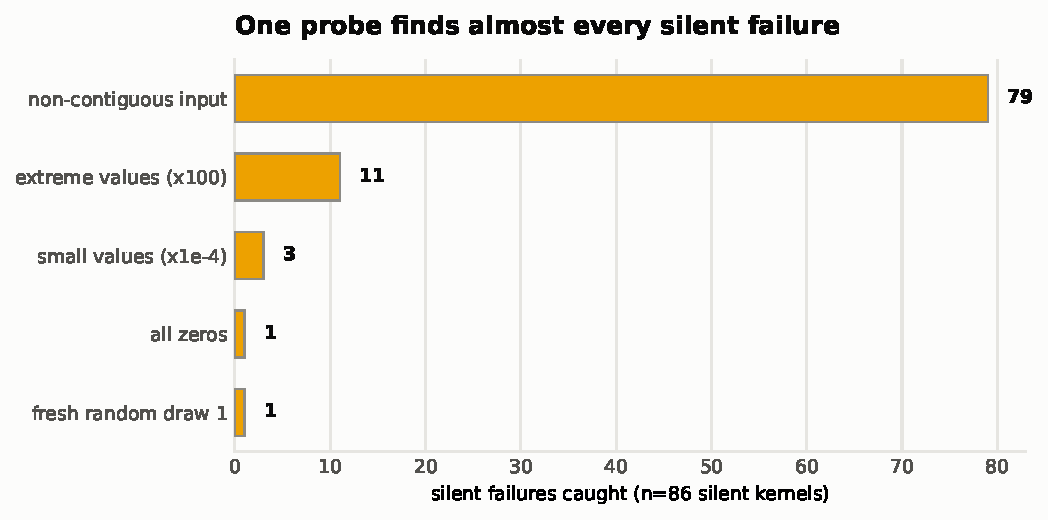
\includegraphics[width=0.88\linewidth]{figures/fig4_probes.pdf}
\caption{Attribution of silent failures to probes. One probe dominates.}
\label{fig:probes}
\end{figure}

The non-contiguous probe is involved in 158 of the 172 silent attempts, and is
the \emph{only} probe that fires in 146 of them, or 85\%. The extreme-value
probe accounts for most of the remainder at 21 attempts. The small-magnitude,
zero and repeated-draw probes contribute almost nothing.

I state this plainly because it is the strongest objection to the work. The
headline finding rests largely on a single relation, that a kernel must not
change its answer when the same values arrive through different strides.

Two pieces of evidence suggest the probe is discriminating rather than a
blanket penalty. It is passed by the large majority of generated kernels, so it
does not simply condemn everything. And the fix is one line, since a kernel
that calls \texttt{.contiguous()} on its inputs satisfies it, which some models
already do unprompted. The probe separates kernels that handle strides from
kernels that assume them away, and that distinction is real.

Even so, a reviewer may fairly say that these kernels satisfy KernelBench's
stated contract, which promises only contiguous inputs. That is why every
false-pass number in this chapter is also reported under the strict reading,
and why Section~\ref{sec:limitations} treats the dependency as a threat to
validity rather than a detail.

\subsection{Cross-GPU divergence}
\label{sec:crossgpu}

Running every kernel on two GPU generations allows a further question: does the
same kernel behave differently on different hardware? Of the 1{,}404 kernels
classified on both an L4 and a T4, 55 received different labels.

Almost all of these are reshuffles among visible failures, such as a kernel
that crashes on one device and returns a wrong answer on the other. Nine
involve a harness fault rather than the kernel. Exactly one pair looked like
the case of real interest, a kernel passing on one device and silently failing
on the other, and inspection shows it is an artefact: on the 16\,GB T4 all
eight probes were skipped for lack of memory, so the battery never ran and the
kernel was recorded as passing without being tested.

The honest conclusion is therefore negative. \textbf{No kernel in this dataset
genuinely passed on one GPU and silently failed on the other.} Silent failures
are a property of the code rather than of the device, at least across these two
architectures. This is a useful thing to know, because it means the false-pass
rates reported above are not an accident of hardware, but it is not a
contribution and I do not present it as one.

\subsection{Performance of passing kernels}

The last question is whether the kernels that survive are worth having.
Figure~\ref{fig:speedup} shows the distribution of speedups over PyTorch for
passing kernels.

\begin{figure}[htbp]
\centering
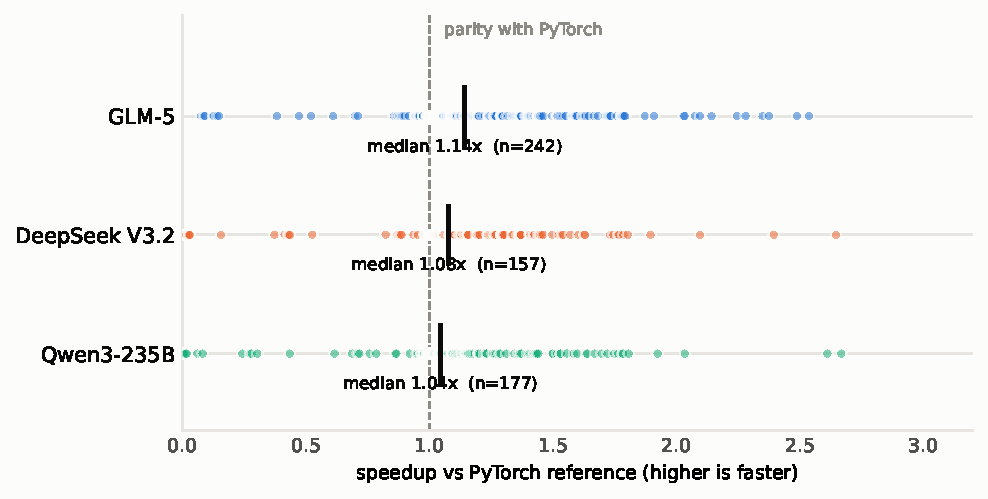
\includegraphics[width=0.9\linewidth]{figures/fig5_speedup.pdf}
\caption{Speedup over the PyTorch baseline for kernels that pass the full
battery. The median gain is small for every model.}
\label{fig:speedup}
\end{figure}

The gains are modest. Median speedups are 1.14$\times$ for GLM-5,
1.07$\times$ for DeepSeek V3.2 and 1.04$\times$ for Qwen3-235B, and between
76\% and 83\% of passing kernels beat PyTorch at all. There is an
uncomfortable pattern here: Qwen3-235B is the most correct model and the
slowest, which suggests that correctness and speed are being traded against
each other rather than achieved together.

One result must be reported separately because it is a flaw in the benchmark
rather than a property of any model. Level 2 problem 80,
\texttt{80\_Gemm\_Max\_Subtract\_GELU}, is degenerate: its output is identically
zero for every input. GLM-5's reasoning arm proved this in a comment and
returned a zero tensor, which is a correct implementation of the specified
module and ran 2{,}671$\times$ faster than PyTorch on the L4 and 6{,}514$\times$
faster on the T4. The kernel is not cheating. The task is broken.

I exclude this problem from the speedup statistics above, and report it here
because anyone quoting KernelBench speedups should know that a single
degenerate task can move an average by a large amount.

%%%%%%%%%%%%%%%%%%%%%%%%%%%%%%%%%%%%%%%%%%%%%%%%%%%%%%%%%%%%%%%%%%%%%%%%%%%%%%%%
% 6. LIMITATIONS -- 2 pages
%%%%%%%%%%%%%%%%%%%%%%%%%%%%%%%%%%%%%%%%%%%%%%%%%%%%%%%%%%%%%%%%%%%%%%%%%%%%%%%%
\section{Limitations and Threats to Validity}
\label{sec:limitations}

\textbf{The stress battery is also an incomplete oracle.} The argument of this
dissertation is that KernelBench decides correctness with a procedure that
cannot see certain faults. Exactly the same criticism applies to the battery.
It inspects seven transformations, and a kernel whose fault appears only under
an eighth will be recorded as passing. Every false-pass rate reported in
Chapter~5 is therefore a \emph{lower bound} on the true rate, not an estimate
of it. This does not weaken the finding, because a lower bound that rises under
repair still shows that repair hides faults, but it does mean the numbers
should be read as ``at least this many'' rather than as a measurement of how
much wrong code exists.

\textbf{One probe carries most of the result.} As Section~\ref{sec:probes}
reports, the non-contiguous probe is the only probe that fires in 85\% of
silent failures. The finding depends heavily on a single metamorphic relation.
A reviewer may reasonably object that KernelBench promises contiguous inputs,
so a kernel that assumes them satisfies the contract it was given. I accept
that this reading is defensible, which is why every false-pass number is also
reported under the strict definition, where such kernels are not condemned. The
two readings disagree about the size of the problem. They agree about its
direction, because the ranking result in Section~\ref{sec:ranking} holds under
both.

\textbf{The study has no confidence intervals.} Temperature is zero and one
sample is drawn per problem, per arm, per turn, so each cell of the design is a
single greedy generation. This makes the experiment exactly reproducible and
cheap, but it means a reported rate such as 20.3\% has no error bar, and a
difference of two or three points between two cells cannot be called
significant. Two things partly compensate. The design is paired, so comparisons
\emph{between} models over the same problems can be tested, and
Section~\ref{sec:ranking} does exactly that with McNemar tests. The relocation
effect also replicates independently across three models and two GPUs, which is
a weaker form of evidence than a confidence interval but not a negligible one.
Drawing five samples per problem for one model would close this gap and is the
first piece of further work I would do.

\textbf{\texttt{compute-sanitizer} never ran.} Stage 2b reports
\texttt{Device not supported} on both GPUs available through Modal, so memory
races and out-of-bounds reads that do not crash the program went undetected
throughout. This is uncomfortable for a study about silent failures, because
some kernels labelled \texttt{pass} or \texttt{silent} may hold memory faults
that a working sanitizer would have raised as \texttt{runtime}. The direction
of the error is not obvious: such kernels might have been reclassified as loud
failures, which would lower the false-pass rate, or the sanitizer might have
exposed further silent faults, which would raise it. I could not run the stage
on the hardware available and I do not know which.

\textbf{The scope is narrow in three ways.} Only Level 2 of KernelBench was
used, so every claim should be read as applying to operator fusion rather than
to whole architectures. Only three models were evaluated, and they were chosen
because their reasoning can genuinely be switched off, which restricts the
findings to models that expose reasoning as a runtime parameter. All three were
served through a single provider, and one of them through an alias,
\texttt{deepseek.v3-v1:0}, that the provider repoints to newer checkpoints over
time. The pipeline did not record which checkpoint answered, so that model is
identified by documentation rather than by captured evidence.

\textbf{The repair loop is one design among many.} Three turns, one prompt
format, and feedback consisting of the compiler message or the numerical
mismatch. A loop that returned richer feedback, or that ran for ten turns,
might relocate more failures or fewer. What this study establishes is that
relocation happens under a plausible and widely used configuration, not that it
happens under all of them.

%%%%%%%%%%%%%%%%%%%%%%%%%%%%%%%%%%%%%%%%%%%%%%%%%%%%%%%%%%%%%%%%%%%%%%%%%%%%%%%%
% 7. CONCLUSION -- 3 pages
%%%%%%%%%%%%%%%%%%%%%%%%%%%%%%%%%%%%%%%%%%%%%%%%%%%%%%%%%%%%%%%%%%%%%%%%%%%%%%%%
\section{Conclusion and Future Work}

\subsection{Summary of findings}

Repair works by the measure the field uses, and that measure is not trustworthy
after repair has been applied.

Across 2{,}852 classified kernels, iterative repair raised the pass rate for
every model in every condition, by as much as 33 points. It raised the
false-pass rate at the same time. In the reasoning arm the share of apparently
correct kernels that fail the stress battery rose from 14.6\% to 20.3\% for
GLM-5, from 17.2\% to 19.6\% for DeepSeek V3.2, and from 7.0\% to 9.8\% for
Qwen3-235B. Counting whole chains rather than rates makes the effect plainer:
of the 244 chains that repair converted into a benchmark success, 79 ended as
silent failures.

The mechanism is not mysterious. A repair loop returns compiler errors, crashes
and failed comparisons, and returns nothing about memory layout. The model
fixes what it is shown. In a typical relocation a kernel fails with an
undefined name, which is about as loud as a failure can be, and returns one
turn later as a kernel that builds, runs, matches the reference on the standard
input and is wrong on a strided one. Both \citet{olausson2024selfrepair} and
\citet{huang2024cannot} predict this, the first because repair is bounded by
the quality of its feedback and the second because improvement measured against
a visible signal is not evidence of correctness. What this work adds is the
measurement.

A second result follows from the first. After repair the three models sit
between 91.5\% and 93.5\% under KernelBench's own contract, and no pairwise
test distinguishes them. Under the stress battery they remain clearly
separated, and their order reverses. Repair does not only inflate the score. It
removes the benchmark's ability to tell good models from weaker ones.

Two smaller results are worth recording. No kernel in this dataset genuinely
passed on one GPU architecture and failed silently on the other, so silent
failure is a property of the code rather than of the device. And Level 2
problem 80 is degenerate, returning zero for every input, which one model
detected and exploited for a speedup above 6{,}000$\times$. That is a flaw in
the benchmark and it affects anyone quoting its performance figures.

\subsection{Conclusions against the objectives}

Objective~1 was met. The classifier assigns one of five categories to every
kernel and was validated against eleven kernels of known category on real
hardware, alongside 86 unit tests. That validation caught three defects which
would each have corrupted the headline number, including one that had silently
disabled the study's principal probe.

Objective~2 was met. The battery encodes seven metamorphic relations, and its
results are withheld from the repair prompt, so a silent kernel ends its chain
without the model ever learning that a probe disagreed. This is what makes the
false-pass rate a measurement rather than a record of how quickly a model can
fit a held-out test.

Objective~3 was met in full. Every one of the 100 Level 2 problems was run for
three models, in two arms, on two GPU architectures, for up to four turns, with
no missing cells.

Objective~4 was met, with a qualification. The ranking does change, and the
change is caused by repair, since both readings agree at turn~0. The strict
half of that result, that the models become statistically indistinguishable, is
established with $p > 0.52$ in every pair. The extended half, that Qwen3-235B
leads, is consistent across both GPUs but reaches significance only when the
two devices are pooled, which overstates the evidence. I report it as a
direction rather than a settled ordering.

Objective~5 was met. The dataset, the kernel sources and the analysis scripts
are released, and no figure or table in this report contains a hand-copied
number.

The aim stated in Section~\ref{sec:aim} can therefore be answered. Repair
improves benchmark scores, and part of that improvement is the disappearance of
evidence rather than the correction of a fault. A repaired kernel is not
reliably more correct. It is reliably harder to catch.

\subsection{Future work}

\textbf{Confidence intervals.} The clearest gap is the single greedy sample per
cell. Drawing five samples at a non-zero temperature for one model in the
reasoning arm would put error bars on the false-pass rate and settle the
ranking question. This needs no new code and roughly one to two days of
compute, and it is the first thing I would do.

\textbf{Feed the battery back on purpose.} This study withholds stage 4 so that
the measurement survives. The opposite experiment is now well defined and
interesting: reveal the battery to the model and measure how many turns it
takes to satisfy it. If the false-pass rate collapses within one or two turns,
that is evidence the model is fitting the probes rather than learning to
respect strides, and it would put a number on how fragile any fixed oracle is.

\textbf{A wider battery.} Because the battery is itself an incomplete oracle,
every rate reported here is a lower bound. Adding relations, for example over
batch size, non-contiguous outputs and mixed dtypes, would tighten that bound
and reduce the dependence on the single relation that currently carries 85\% of
the result.

\textbf{Level 3 and other hardware.} Extending to whole architectures would
test whether relocation survives at greater kernel complexity, and running on a
platform where \texttt{compute-sanitizer} is supported would close the largest
methodological gap in the classifier.

\textbf{A benchmark that reports both numbers.} The practical recommendation
from this work is small and cheap. A kernel benchmark should report the pass
rate together with the share of passes that survive a stress battery. The
second number costs a few seconds per kernel, and without it a repair loop can
raise the first number by hiding faults, with nothing in the report to show it.

%%%%%%%%%%%%%%%%%%%%%%%%%%%%%%%%%%%%%%%%%%%%%%%%%%%%%%%%%%%%%%%%%%%%%%%%%%%%%%%%
% BIBLIOGRAPHY -- outside the 40 page limit
%%%%%%%%%%%%%%%%%%%%%%%%%%%%%%%%%%%%%%%%%%%%%%%%%%%%%%%%%%%%%%%%%%%%%%%%%%%%%%%%
\bibliographystyle{apalike}
\bibliography{kfault}

%%%%%%%%%%%%%%%%%%%%%%%%%%%%%%%%%%%%%%%%%%%%%%%%%%%%%%%%%%%%%%%%%%%%%%%%%%%%%%%%
% APPENDICES -- 3 pages, INSIDE the 40 page limit
%%%%%%%%%%%%%%%%%%%%%%%%%%%%%%%%%%%%%%%%%%%%%%%%%%%%%%%%%%%%%%%%%%%%%%%%%%%%%%%%
\newpage
\appendix

\section{Generation and Repair Prompts}
% TODO verbatim prompt text.

\section{Per-Problem Results}
% TODO tables from data/attempts.csv.

\section{A Degenerate KernelBench Task}
% TODO task 80 kernel source.

\end{document}
